\documentclass{article}
\usepackage[utf8]{inputenc}
\usepackage{mathtools}
\usepackage{graphicx}
\graphicspath{ {1_One_Uncertain_EF} }

\title{Analysis of uncertainties in emission inventories with Markov Chain Monte Carlo}
\author{Bart Degraeuwe, Emanuela Peduzzi}
\date{September 2019}

\begin{document}

\maketitle

\section{Introduction}
Emissions inventories provide, for a given area, the total emissions of several pollutants per sector. Typical pollutants are (\(CO_{2}\)), particulate matter (PM), volatile organic compounds (VOC), nitrogen oxides (\(NO_{x}\)) and ammonia (\(NH_{3}\)). some examples of sectors are power generation, industry, domestic heating and transport. Inventories are built with estimates of the activity level in the sector and emission factors for the different pollutants. Activity levels quantify the activities responsible for emissions, e.g. energy consumption for heating in the residential sector or distance travelled by type of vehicle for transport. If for the area of interest the activity is not know it can be derived from a national total and a proxy. E.g. population and road network density can be used as a proxy for transport. The activity level in the area of interest is the product of the national total and the value of the proxy in the area. The product of the activity level and the corresponding emission factor per pollutant yields the spatially distributed emissions provided by an emission inventory. 
However, different inventories in a given area do not usually agree and provide different estimates for the pollutant emissions of a sector. All pollutant emissions of a sector share the same activity and use a specific emission factor for the respective pollutants. Hence, the variability in emissions between pollutants and inventories might tell something about the underlying cause. Two examples:
\begin{enumerate}
\item It is possible to infer that, if several inventories agree on the emissions of all pollutants but one, there is high uncertainty on the emission factor of that one pollutant. On the other hand, if one inventory provides consistently different emissions of a given sector for all pollutants with respect to the other inventories, it is reasonable to assume that the culprit is the activity level of that inventory – sector combination.
\item It may happen that there is a big variability in emissions but the same inventories are systematically over or underestimating the emission for each pollutant. In this case it is likely that the activity is uncertain.
\end{enumerate}
The question that we would like to answer is therefore “\textbf{What does the variability in the emissions of different inventories tell us about the uncertainty of the underlying activity and emission factors?}”
It is reasonable to assume that neither the activity nor the emission factors of the different sectors are related. Hence, the analysis can be limited to one sector for which the emissions of a number of pollutants are provided by several inventories. We would like to know if the variability in the total emissions is rather due to the uncertainty of the activity or rather due to the uncertainty of the emission factors. To provide an answer we built a stochastic model of the problem, we did a simulation study, and finally we applied the model to real data. 
\section{A stochastic model of the uncertainties in activity, emission factors and emissions}
The emissions \(E_{ij}\) provided by each inventory \textit{i} for a pollutant \textit{j} are the product of the activity \(AC_{i}\) and an emission factor \(EF_{ij}\). The activities and emission factors are unknown. But we know that each inventory uses the same activity for all the pollutants and multiplies it with the corresponding emission factors. Different inventories use different emission factors for the same pollutant.
\[E_{ij}=AC_{i} . EF_{ij}\]
\(\forall i \in [1,V]\) with V the number of inventories and \(\forall j \in [1,P]\) with P the number of pollutants.

Emission factors and activities are always positive. Hence, it makes sense to assume they follow a log-normal distribution. So, their logarithms are normally distributed. We work with the logarithms from now on.
\[log(E_{ij})=log(AC_{i})+log(EF_{ij})\]
The logarithms of the activities used in each inventory are assumed to be normally distributed around the logarithm of real unknown activity, \(\mu_{\log(AC)}\), with an unknown standard deviation \(\sigma_{\log(AC)}\).
\[\log(AC) \sim N(\mu_{\log(AC)},\sigma_{\log(AC)})\]
Similarly, the emission factor of each pollutant is log-normally distributed around \(\mu_{log(EF_{j})}\) with standard deviation \(\sigma_{log(EF_{j})}\): 
\[\log(EF_{j}) \sim N(\mu_{\log(EF_{j})}, \sigma_{\log(EF_{j})})\]

Of course we would like to know the real \(\mu_{\log(AC)}\)  and \(\mu_{\log(EF_{j})}\) but we only have estimates of their sum, i.e. the logarithm of the emissions. We cannot undo this sum. Anyway, we are interested in the relative standard deviations of activities and emission factors. They are related to the standard deviations of the logarithms of activity and emission factors.

This is a property of the log-normal distribution. Assume X is normally distributed with mean \(\mu\) and standard deviation \(\sigma\). Then \(Y=\exp{X}\) is log-normally distributed with expected value \(E(Y)=\exp(\mu+\frac{\sigma^2}{2})\) and standard deviation \(\sqrt{(\exp(\sigma^2)-1)\exp(2\mu+\sigma^2}\). The relative standard deviation of Y is:
\[\frac{\sqrt{Var(Y)}}{E(Y)} = \frac{\sqrt{\exp(\sigma^2)-1}.\exp(\mu+\sigma^2/2)}{\exp(\mu+\sigma^2/2)} = \sqrt{\exp(\sigma^2)-1}\]
This means that the relative uncertainty (or relative standard deviation) of the activity depends only on the standard deviation of the logarithm of the activity. The same is true for the emission factors. Now we will define a stochastic model for the relative uncertainties of activity and emission factors using the total emissions of several pollutants and inventories.

The stochastic model links the response, the logarithm of the emissions of P pollutants for V inventories, to expected values and standard deviations of the activity and emission factors. The response is normally distributed around a pollutant specific value \(\mu_{\log(E_{j})}\) with a precision \(\tau\). The precision is the inverse of the variance.
\[\log(E_{ij}) \sim N(\mu_{log(E_{j})},\tau_{j})\]
The variance of an emission estimate of a pollutant is the sum of the variance of the activity and the variance of the emission factor of that pollutant. This is only true if the activity and emission factors are independent samples. This hypothesis will be discussed later.
\[Var(\log(E_{ij})) = Var(\log(AC)) + Var(log(EF_{j}))\]
Or terms of precisions this means:
\[\tau_{j} = \left(\tau_{log(AC)}^{-1} + \tau_{log(EF_{j})}^{-1}\right)^{-1}\]
The precision gives a nested structure to the model. The precision of the activity is shared by all inventories and pollutants. The precision of an emission factor is shared by all emissions of the same pollutant.
We will use Markov Chain Monte Carlo (MCMC) to find a solution for \(\mu_{log(E_{j})}\), \(\tau_{log(AC)}\) and \(\tau_{log(EF_{j})}\). Therefor we need to define priors. As prior for \(\mu_{log(E_{j})}\) the average of the logarithms of the emission of a pollutant is chosen with an uninformative low precision.
\[\mu_{log(E_{j})} \sim N\left(\frac{1}{V}\sum_{i=1}^{V} \log(E_{ij}),10^{-4}\right) \]
For the precision of the activity and the emission factors uninformative gamma priors are used:
\[\tau_{log(AC)} \sim \Gamma(10^{-4},10^{-4})\]
\[\tau_{log(EF_{j})} \sim \Gamma(10^{-4},10^{-4})\]
Figure \ref{fig:graph} shows the acyclic graph of the model. Squares represent known values. Circles are stochastic nodes, i.e. variables that follow a specified distribution. Dashed circles are computed nodes. The arrows indicate dependencies.
In the next section this model will be applied to some synthetic examples.

\begin{figure}
    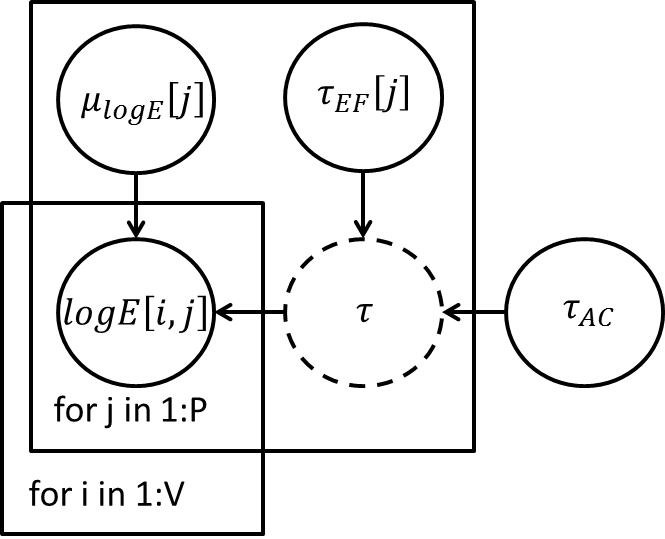
\includegraphics[width=4.5in]{acyclic_model_graph.png}
    \caption{Acyclic graph of the emission uncertainties model.}
    \label{fig:graph}
\end{figure}

\section{Simulation studies}
To assess what can be expected from methodology described above some simulation studies are presented. In a simulation study activity levels and emission factors are drawn from known distributions for a chosen number of inventories. The expected values of the distributions can be chosen freely. They have no impact on the results. Of interest are different combinations of relative standard deviations for activity and emission factors. Then the emissions are calculated multiplying the randomly generated activities and emission factors. Actually their logarithms are summed. The methodology described above is then applied to these simulated emissions. The results are distributions for the standard deviations of \(\log(AC)\) and \(\log(EF_{j})\). From the latter a distribution of the ratios of relative standard deviations of AC and EFp can be calculated with formula:
\[\forall j \in [1,P]:  \frac{\frac{\sigma_{AC}}{\mu_{AC}}}{\frac{\sigma_{EF_{j}}}{\mu_{EF_{j}}}} = \sqrt{\frac{2\exp{\sigma_{logAC}}+1}{2\exp{\sigma_{logEF_{j}}}+1}}\]
The resulting distribution can be compared with the original input to check if it’s possible to find the input back.

\subsection{One more uncertain emission factor}
Emissions are simulated assuming that the emission factor of one pollutant has a higher relative uncertainty than the activity and other emission factors. There are 7 inventories and 4 pollutants. These numbers were chosen because the real data, presented in the next section, have this structure. Table \ref{tab:one_uncertain_EF} shows the relative uncertainties of activity and emission factors.

\begin{table}[h]
\begin{tabular}{llllll}
& AC   & EF1  & EF2  & EF3  & EF4  \\
relative std. dev. & 10\% & 10\% & 10\% & 10\% & 20\%
\end{tabular}
\caption[Relative standard deviations for a simulation study with a more uncertain emission factor for pollutant 4]{Relative standard deviations for a simulation study with a more uncertain emission factor for pollutant 4} 
\label{tab:one_uncertain_EF}
\end{table}



\begin{figure}[h]
    \includegraphics[width=4.5in]{One_uncertain_EF/Hist_Ranking.png}
    \caption{PDF of the standard deviations of activity and emission factors for one more uncertain emission factor}
    \label{fig:One_uncertain_EF}
\end{figure}

\end{document}
